First of all we introduce the hierarchy of data structures with respect to persistence.

\begin{itemize}
\item {\bfseries Ephemeral data structures} Past states are destroyed by new changes and irretrievably lost.
\item {\bfseries Semi-persistent data structures} (Sometimes partially persistent) Past states are stored and can be accessed for reading, modifying operations are only allowed on the most recent version. Operations produce return a new version handle. Historical versions form a linear order.
\item {\bfseries (Fully-)persistent data structures} Versions form a rooted tree, additional changes can be made to any existing version, creating a new version as a child vertex.
\item {\bfseries Functional data structures} No changes are permitted to written data.
\end{itemize}

This division is by no means universally adopted, but provides an interesting perspective regardless.

With a persistent data structure, we essentially want to have one data structure for every existing version. Insert and delete return a new version handle instead of making changes to the existing version. Obviously, copying the data structure every time is one option how to achieve this, albeit not a great one. To prevent using extra memory and increased time complexity of operations however, more intricate methods must be employed.

Going beyond this hierarchy, if fully-persistent data structure also supports merging or melding two different versions, it is called \textit{confluently persistent} \cite{confluently-persistent}. We will not investigate confluent persistence in this thesis further.

\section{Persistence through Path-Copying}

Binary search tree can be converted into a fully-persistent one rather easily.
One possible approach is called path-copying. It is based on the observation that most of the tree does not change during an operation.

When a new version of the tree should by created by delete or insert, new copies are allocated only for vertices that are changed by the operation and their ancestors. This typically means that only path from the inserted/deleted vertex to the root is newly allocated, plus constant number of other vertices. The new vertices carry pointers to the old vertices where subtree rooted at such a vertex is not modified in any way.

With reasonable variants of binary search trees, achieved time complexity in a tree with $n$ vertices is $\Theta(\log n)$ per operation and $\Theta(\log n)$ memory for insert/delete.

The downside of this method is the increased memory complexity. There is no known construction that would not increase memory complexity by copying the paths.

\section{Multiple versions in one vertex}

To limit memory consumption we may rather choose to let vertices carry their properties for all versions. This in reality means that we must store a collection of changes together with versions when they happened. 

When we arrive at a vertex asking for the state in version $A$, we must go through the collection of changes to figure out what the state in version $A$ should be. In fact, it will be easier to just copy all of the other fields the vertex possesses as well if one of them changes. One change will therefore hold new values for all fields of the vertex. The issue of how to effectively determine which changes should be applied will be addressed later through introduction of total ordering of all versions.

Looking at the memory consumption, it appears clear that the amount consumed stems from the total number of changes done by the balancing algorithm across all operations.

What remains to solve though is to choose the right kind of collection for versions of changes for one vertex. Surely using linked lists or arrays will inevitably lead to unsatisfactorily inefficient processing of applicable changes. Unfortunately as it turns out, even other data structures will let us down here.

With this approach, we can reach linear memory complexity (with the total number of changes). On the other hand execution time will be hurt. We can reach the following amortized complexity depending on the chosen data structure:

\begin{tabular}{ll}
Linked list & \bigO{n \log n} \\
Binary search tree & \bigO{\log^2 n} \\
Q-fast trie & \bigO{\log ^{3/2} n}, semi-persistence only \\
Y-fast trie & \bigO{\log n \cdot \log \log n}, semi-persistence only, on average

\end{tabular}

\begin{figure}
	\begin{center}
		\begin{tikzpicture}[sibling distance=8pt]
		\Tree[
		.B A [ .C \edge[blank]; \node[blank]{}; D ]
		]
		\node at (0,1) {Version 1};
		\end{tikzpicture}
		\qquad\hspace{40mm}
		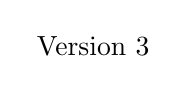
\begin{tikzpicture}[sibling distance=8pt]
		\Tree[
		.B A [ .D C E ]
		]
		\node at (0,1) {Version 3};
		\end{tikzpicture}
	\end{center}
\raggedcolumns
\begin{multicols}{2}
\centering
\footnotesize
\begin{vdTable}{Vertex}
	Version & Left & Right   & Key & Value
\end{vdTable}
\begin{vdTable}{A}
	1 & $\Lambda$ & $\Lambda$ & 10 & 5 \\
	2 & $\Lambda$ & $\Lambda$ & 10 & 6
\end{vdTable}
\begin{vdTable}{B}
	1 & A & C & 20 & 15 \\
	3 & A & D & 20 & 15
\end{vdTable}
\begin{vdTable}{C}
	1 & $\Lambda$ & D & 30 & 27 \\
	3 & $\Lambda$ & $\Lambda$ & 30 & 27
\end{vdTable}
\begin{vdTable}{D}
	1 & $\Lambda$ & $\Lambda$ & 40 & 39 \\
	3 & C & E & 40 & 39
\end{vdTable}
\begin{vdTable}{E}
	3 & $\Lambda$ & $\Lambda$ & 50 & 99
\end{vdTable}\\
\end{multicols}

{\small
Tree is shown for version 1 (left) and 3 (right). 
Internal collections for each vertex are displayed. 
Operation that created version 2 changed value of key 10. Operation that created version 3 inserted vertex E and triggered a rotation. 
Faithful to The Art of Computer Programming, $\Lambda$ represents a null pointer.
}

\caption{A tree with dictionaries in vertices} 

\end{figure}

\section{Fat Vertices}

Following up on the idea of multiple versions in one vertex, fat vertices were devised. We will explain this technique only for semi-persistence first. Full persistence requires the use of a few extra tricks and ordering on the versions.

A fat vertex stores is generally a dictionary of standard vertices indexed by versions. We call values of this dictionary slots. The maximum size of this dictionary is set to a constant which is determined later. Instead of copying the vertex, we simply add new version into the dictionary. This stops the propagation of changes toward the root, provided the maximum has not been exceeded yet. Because of the limit on size of this dictionary, it may be implemented simply as a linked list.

Contents of one slot are a version handle, all pointers a vertex would have, then inverse pointers to fat vertices that have slots pointing to this fat vertex for this version and 
some fields, notably key and value. Not all fields need to be versioned. For example balancing information may be stored only for the latest version, i.e. in red-black trees color is only used for balancing and is thus not needed to be available for old versions. 

One vertex in the original binary search then corresponds to a doubly-linked list of fat vertices. When the vertex should change, new state of the vertex is written into a slot of the last fat vertex in the list. As all slots become occupied in the last fat vertex and it needs to be modified, new vertex is allocated.

Modifications of a single vertex during one operation are all written to single slot, there is no need for using more slots.

When a new fat vertex $x$ is allocated, one of its slots is immediately taken. Pointers must be updated in other fat vertices that pointed to the fat vertex preceding $x$ in the list. This is done either by inserting new slot into them (copying all values from the latest slot and replacing pointers to the predecessor by pointers to $x$.). Or by directly updating the pointers if the version is already present. 

Recursive allocations may be triggered, which is not a problem if there is only a small amount of them. This is ensured by setting the size of fat vertices suitably. We can place an upper bound on the number of newly allocated fat vertices -- total number of vertices in the tree (including deleted vertices). At most one new slot is occupied for every vertex in the tree.

To take advantage of fat vertices, we need the balancing algorithm to limit the number of vertices that change in one operation. This was the goal of modified WAVL-balancing algorithm all along. Furthermore, we need a limit on pointers that can target one vertex at one time.

Temporarily, we will allow the capacity of fat vertex to be exceeded. This will have to be fixed however, before the ongoing operation finishes.

\begin{prop}
Suppose any binary search tree balancing algorithm satisfying the following properties:
\begin{itemize}
\item 
There is a constant $k$ such that for any $n$ successive operations on initially empty tree, the number of vertex changes made to the tree is at most $kn$. 
\item 
There is a constant bound on the number of pointers to any one vertex at any time.
\end{itemize}
Then this algorithm with the addition of fat vertices for semi-persistence, consumes $\mathcal{O}(n)$ space for the entire history of $n$ operations starting from an empty tree.
\end{prop}

\begin{myproof}
We denote the number of pointer fields per vertex as $p$ and maximum number of vertices pointing to one vertex at a time as $x$. We then define the number of slots in fat vertex as $s = p + x + 1$ (higher value is also possible).\\
We define the potential of the structure as the sum of numbers of occupied slots in all most recent versions of vertices. (Thus initially zero.) Allocation of new fat vertex will cost one unit of energy. This cost can be charged from the potential or the operation. We will show that the operation needs to by charged only a constant amount of energy per one vertex modification by the original algorithm (to compensate increase in potential or pay for allocations), from which the proposition follows.\\
For insert, a new vertex is created (which increases potential by a constant). During rebalancing of the tree, $r$ vertices are to be modified. Let us consider this sequence of modifications one by one. We send one floating unit of energy to each of the $r$ vertices.\\
If a modification of $v$ is second or later modification of $v$ during this operation, changes are simply written to the slot for this version.\\
Otherwise, number of used slots is checked. If there is one or more empty available, new slot is used, taking default values of fields from preceding slot. This increases potential by one, which is covered by the floating unit of energy.\\
If no slots are available, new fat vertex $v'$ is allocated and one of its slots is used. This decreases potential by $p+x$. The floating unit of energy is used to pay for allocation of the new vertex. Next, fat vertices to corresponding current version interval of vertices having pointers to $v$ need to have this reflected. Additionally inverse pointers to $v'$ need to be set. These are at most $p+x$ changes to other vertices that may use their new empty slots. The decrease in potential is used to send one unit of energy to every such vertex that need an update. Changes are executed recursively and by will not require extra energy to be charged on the operation.
\end{myproof}

Regarding the time complexity, searching the correct slot in a fat vertex produces only constant overhead. Realizing that every operation can be charged on a memory allocation of a fat vertex such that there is a constant $c$ depending only on the balancing algorithm such that for every allocated fat vertex the number of operations charged on it is at most $c$.

\begin{obs}
Assuming the conditions from the previous proposition, the cost to write changes into fat vertices as amortized to \bigO{1} per operation.
\end{obs}

We see that WAVL trees can be used for semi-persistence even in their original form, along with many other binary search trees. Time complexity of operations with the tree depends on the original balancing algorithm used. With WAVL trees we get \bigO{\log n} per operation from the original algorithm in addition to the amortized \bigO{1}. Here $n$ is the size of the tree in the version that is queried.

In fact, for semi-persistence fat vertices may be defined differently. It suffices that only values of changed fields and pointers are written into slots. Thus each fat vertex carries a set of default values for every field and pointer, these values are used if not overridden by a slot. This approach may lead to lower memory consumption and cannot be used for full persistence.

\begin{figure}
	\centering
	\ttfamily
	\begin{tabular}{cccccc}
		Rank  & Previous &  Next   &      & &          \\ \hline
		Left1 &  Right1  & Parent1 & Key1 & Value1 &  Version1 \\ \hline
		Left2 &  Right2  & Parent2 & Key2 & Value2 & Version2 \\ \hline
		Left3 &  Right3  & Parent3 & Key3 & Value3 & Version3 \\ \hline
		Left4 &  Right4  & Parent4 & Key4 & Value4 & Version4 \\ \hline
		Left5 &  Right5  & Parent5 & Key5 & Value5 & Version5 \\ \hline
		Left6 &  Right6  & Parent6 & Key6 & Value6 & Version6 \\ \hline
	\end{tabular}
	\normalfont
\caption{Layout for WAVL semi-persistent tree fat vertex}
\end{figure}

\section{Parallel Semi-Persistence with WAVL Trees}

Insertion and deletion in a WAVL tree can be also carried out top-down\cite{rank-balanced-trees}.
It is also possible to preemptively perform rotations, promotes and demotes when descending to make sure that more changes of high ranks will not be needed. This means that as insert or delete will descend down the tree towards the leaves processing vertices along some path, it will hold locks for vertices in at most constant distance from the vertex that the operation is currently processing.

It can be shown that there at most \bigO{1} modifications of the structure per operation (amortized), albeit the constant proves to be rather high. These facts lay a solid foundation to parallel semi-persistence.

What is unfortunate, is the delete procedure, which must locate an additional vertex to swap values in case of the deleted vertex having two children. So we will assume that delete is not possible for now.

First of all two kinds of operations must be identified. 

\begin{itemize}
	\item Query on any version of the tree (id est find, min, max and range functions)
	\item Insert (into the newest version of the tree)
\end{itemize}

Let us address data races between inserts first. For every insert, prior to all else, new version handle must be created. This is achieved simply by incrementing a version counter which is done in constant time and will not block other threads much. The insert itself follows.

Locking procedure will be this: When we enter a fat vertex, we lock it for other threads of computation. Conversely, lock for a fat vertex is lifted when insert holding the lock  is unlocked by the original algorithm. Since all threads begin locking at the root and descend towards the leaves, no deadlocking is possible among inserts. This follows from the fact that rotations are only done among vertices locked by the same operation.

Applying the algorithm with semi-persistence we must however ensure that before unlocking a fat node, none of its children may run out of slots leading to allocation of a replacement. Since there can be at most one new slot occupied for every fat node in one operation, it suffices to allocate new fat vertex for every fat vertex without empty slots before releasing its parent.

To address queries, we first assume that queries are only started on a version that was generated by already complete insert. In this situation, queries may pass through fat vertices with little regard to ongoing inserts. Queries will thus ignore locks on fat vertices. Only one thing must be considered -- modification of slots by insert (being non-atomic) requires exclusive write lock on the slots that are modified. Queries will require shared read-only lock. Since reading of information from slots by insert may only be obstructed by writing by the same insert, read-only lock is not needed in this case. No deadlocks will arise from this locking can be conducted starting from the head of slots linked list in all cases. 

If we increase the number of slots in a fat vertex by at least one, asymptotic memory consumption remains linear with length of history. Time complexity for one operation remains the same as without this modification for concurrence, that is if time spend being blocked by other threads is excluded.

Let us turn back to enabling delete. If delete operations are rare, we may simply treat them as inserts locking-wise and acknowledge that they blocking may ensue. Another approach would be to use the technique of \textit{ghost vertices}. That is to add a deleted flag to vertex layout, deleting would simply set this flag in corresponding slot. This will increase size of the tree. For the number of deleted vertices bounded by a polynomial in the number of remaining vertices for every version of the data structure, this preserves the asymptotic time complexity. 

Otherwise, an entirely new data structure may be built from the latest versions of all vertices in the tree if the amount of deleted vertices exceeds a certain ratio to remaining vertices. The cost to build this new tree is amortized into the deletes from the preceding data structure.

\section{List Ordering}

Moving from semi-persistence to full-persistence we encounter an obstacle -- versions no longer form implicit linear order. Nonetheless, to work with fat vertices, we need to be able to determine slots that carry values correct for current version. To achieve this, we need to identify an interval of versions the current vesion would fall into. For this we will try to introduce an ordering to versions of the persistent data structure.

Version do form a rooted tree with the original version in the root. We can also order children of every vertex by the order of their creation. (the latest creation first) We then define the desired ordering as the order of vertices corresponding to versions as they are visited by an in-order traversal.

In reality, we will also insert other elements into the ordering that will be helper version and will not be used to represent the state of the entire structure after a sequence of operations. This can be disregarded for now.

With the ordering defined, we still need a way to efficiently represent it in memory. The operation we really need are

\begin{itemize}
	\item InsertSuccessor(Version),
	\item Compare(VersionA, VersionB).
\end{itemize}

To preserve the speed of semi-persistence, \texttt{Compare} must be \bigO{1} and \texttt{InsertSuccessor} \bigO{\log n} at least amortized. Weight-balanced trees that were introduced in the previous chapter are ideally suited for this purpose.

For every vertex in the weight-balanced tree, we will store encoding of the path from root to it in form of sequence of 0s and 1s. 1 for right child, 0 for left child. We know that depth of the tree must be logarithmic. (Here we tacitly assume that arithmetic with numbers of size on the order of number of versions can be done in constant time.) So comparing version is efficient. Inserting a successor version is also straight-forward. Rebuilding of some subtree will not change order of versions as all path encodings will recalculated.

\section{Fully-Persistent WAVL Tree}

Before delving into the details of modified fat vertices for full-persistence, we must note that amortized constant number of changes per operation will no longer suffice. If there exist a version of the structure and an operation that causes large amount of changes to the structure, nothing is stopping us from repeatedly performing this operation on this version, thus consuming super-linear amount of space.

For achieving full persistence, we will build upon the technique of fat vertices. Now however, simply allocating new vertex when we run out of empty slots in the old one will not do. It remains crucial that occupied slots of one fat vertex form an interval of existing versions. In particular, It will be needed to insert between existing versions

\begin{prop}
Suppose any order of splitting fat vertices with the number of slots exceeding the set limit $l$ during an operation on a tree $T$. Regardless of the way for choosing the next node to be split, number of occupied slots in all nodes will remain under .
\end{prop}